\documentclass{scrartcl}
\usepackage{graphicx}
\usepackage{xspace}

%\newcommand{\class}[1]{\textbf{#1}}
\newcommand{\class}[1]{\texttt{#1}}
\newcommand{\kdtub}{\textsc{realKD}\xspace}

\title{---\kdtub---\\Java Library for Real Knowledge Discovery}
\subtitle{Document version 1 \\ (referring to library version 0.1)}
\author{Mario Boley\\University of Bonn/Fraunhofer
IAIS\\Schloss Birlinghoven, Sankt Augustin}

\begin{document}

\maketitle

\section{Introduction}
This document is a developer's guide to \kdtub---a free open-source Java library
that has been designed to help real users discovering real knowledge from real data. 
As such it has a strong focus on
\begin{itemize}
\item[a)] a detailed data model that allows the specification of a lot of
domain-dependent semantics,
\item[b)] a generic pattern model intended to capture meaningful bits of
knowledge, and
\item[c)] a model to describe algorithms and their parameters in a way that
makes it easy to build user-friendly applications on top of it.
\end{itemize}
In particular \kdtub can be used to discover associations (itemset patterns),
exceptional model patterns (subgroups), and subspace outliers from tabular data.
While the main purpose of \kdtub is to be used by other Java applications that
aim to enable knowledge discovery functionality to their users, it can also be used
stand-alone from the command line.

This document gives a brief introduction to the comncepts and interfaces of
the library. It is targeted towards developers who want to use components of
\kdtub to build a data analysis tool on top of it as well as those that want to extend its functionality---either to be included in a future version of this library or
outside of it within other third party software.

% The library consists of
% three parts:
% a data model, pattern definitions, and data mining algorithms.
% 
% The most abstract layer is the data model, which contains interfaces, through
% which data and meta-data is accessed by the rest of the software.
% Currently, data can be expressed in tabular form and in the form of binary
% propositional statements about a set of data objects.
% 
% Then there is the pattern layer for expressing interesting observations that
% can be made in the data. This layer contains pattern descriptors,
% interestingness functions for expressing the usefulness or quality of a pattern, and of course classes for complete pattern definitions of different types. 
% Currently, \kdtub supports association patterns, outlier patterns, and
% exceptional model mining patterns (subgroup mining). 
% 
% Finally, there is
% the layer of mining algorithms, which can discover patterns based on an instance
% of the data model. This layer also contains a model for meta-information of mining
% algorithms, which can be used by clients to control the algorithms and their
% parameters.
% \kdtub contains different algorithms for the discovery of each of the supported
% pattern types. Currently, this includes myopic beam search algorithms as well as
% randomized sampling algorithms.

\begin{figure}[ht]
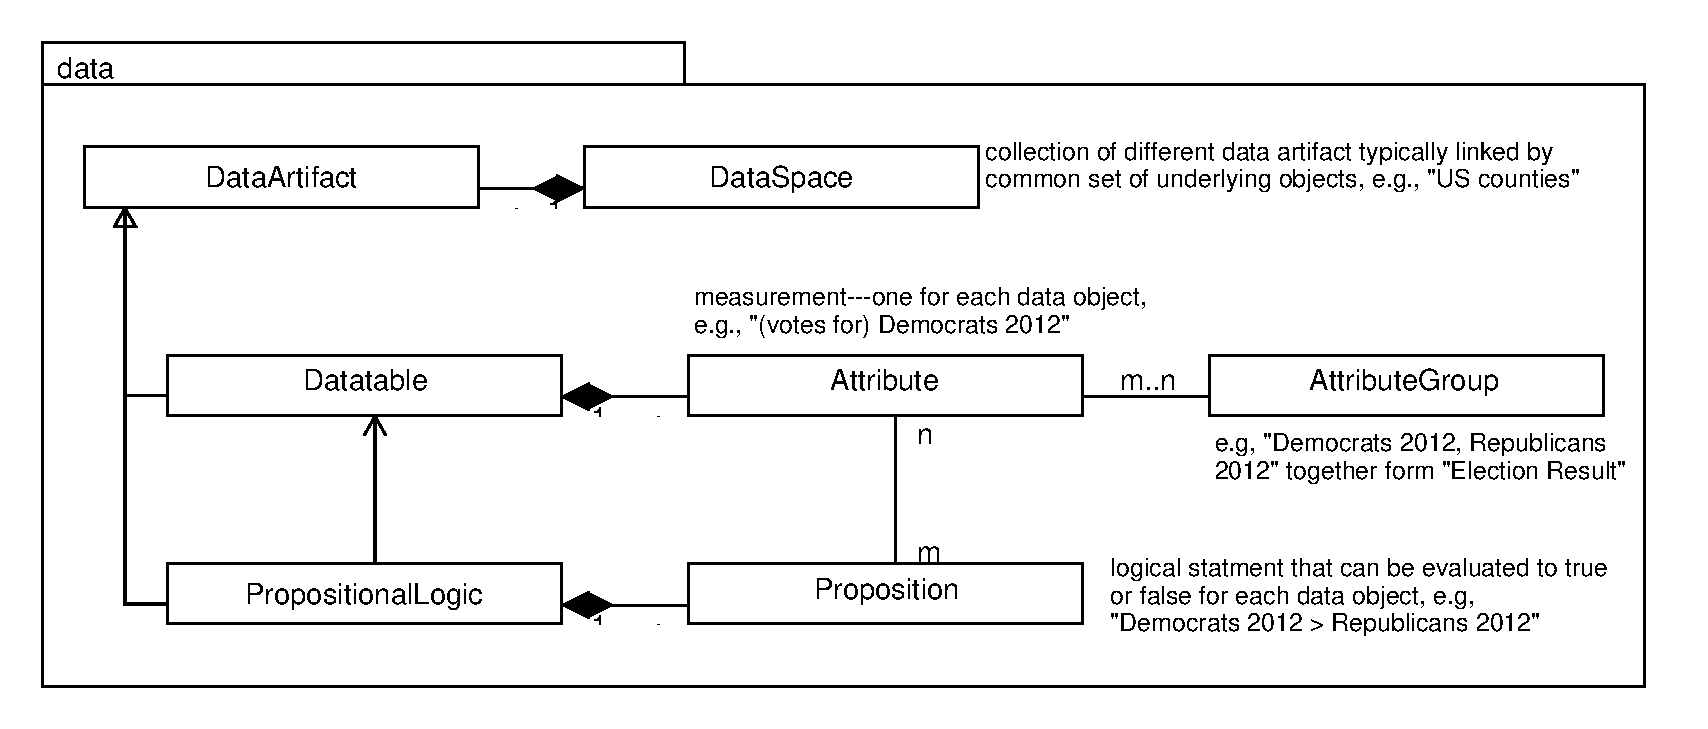
\includegraphics[width=\columnwidth]{data/data_overview.pdf}
\caption{Classes of the tabular data model.}
\label{fig:dataclasses}
\end{figure}
\section{Data Model}
The basic form of input data in \kdtub is tabular. That is, it is given in the
logical form of a table with a fixed number of rows and columns represented by
the main class \class{Datatable}.
A table contains a number of data records (rows), each of which is described by
a fixed set of attributes (represented by the class \class{Attribute}). These
attributes can be categorical (they assign to each data record one of a typically small number of fixed categories), ordinal (same as
categorical but in addition there is a partial order over the categories), or
metric (assign to each data record a double value). Values can be also be
explicitly marked as missing. Additionally, there is
attribute metadata in the form of attribute groups, which stand in an n-to-m
relationship with the attributes. See Fig.~\ref{fig:dataclasses} for a summary
of the classes of the data model.
\begin{figure}
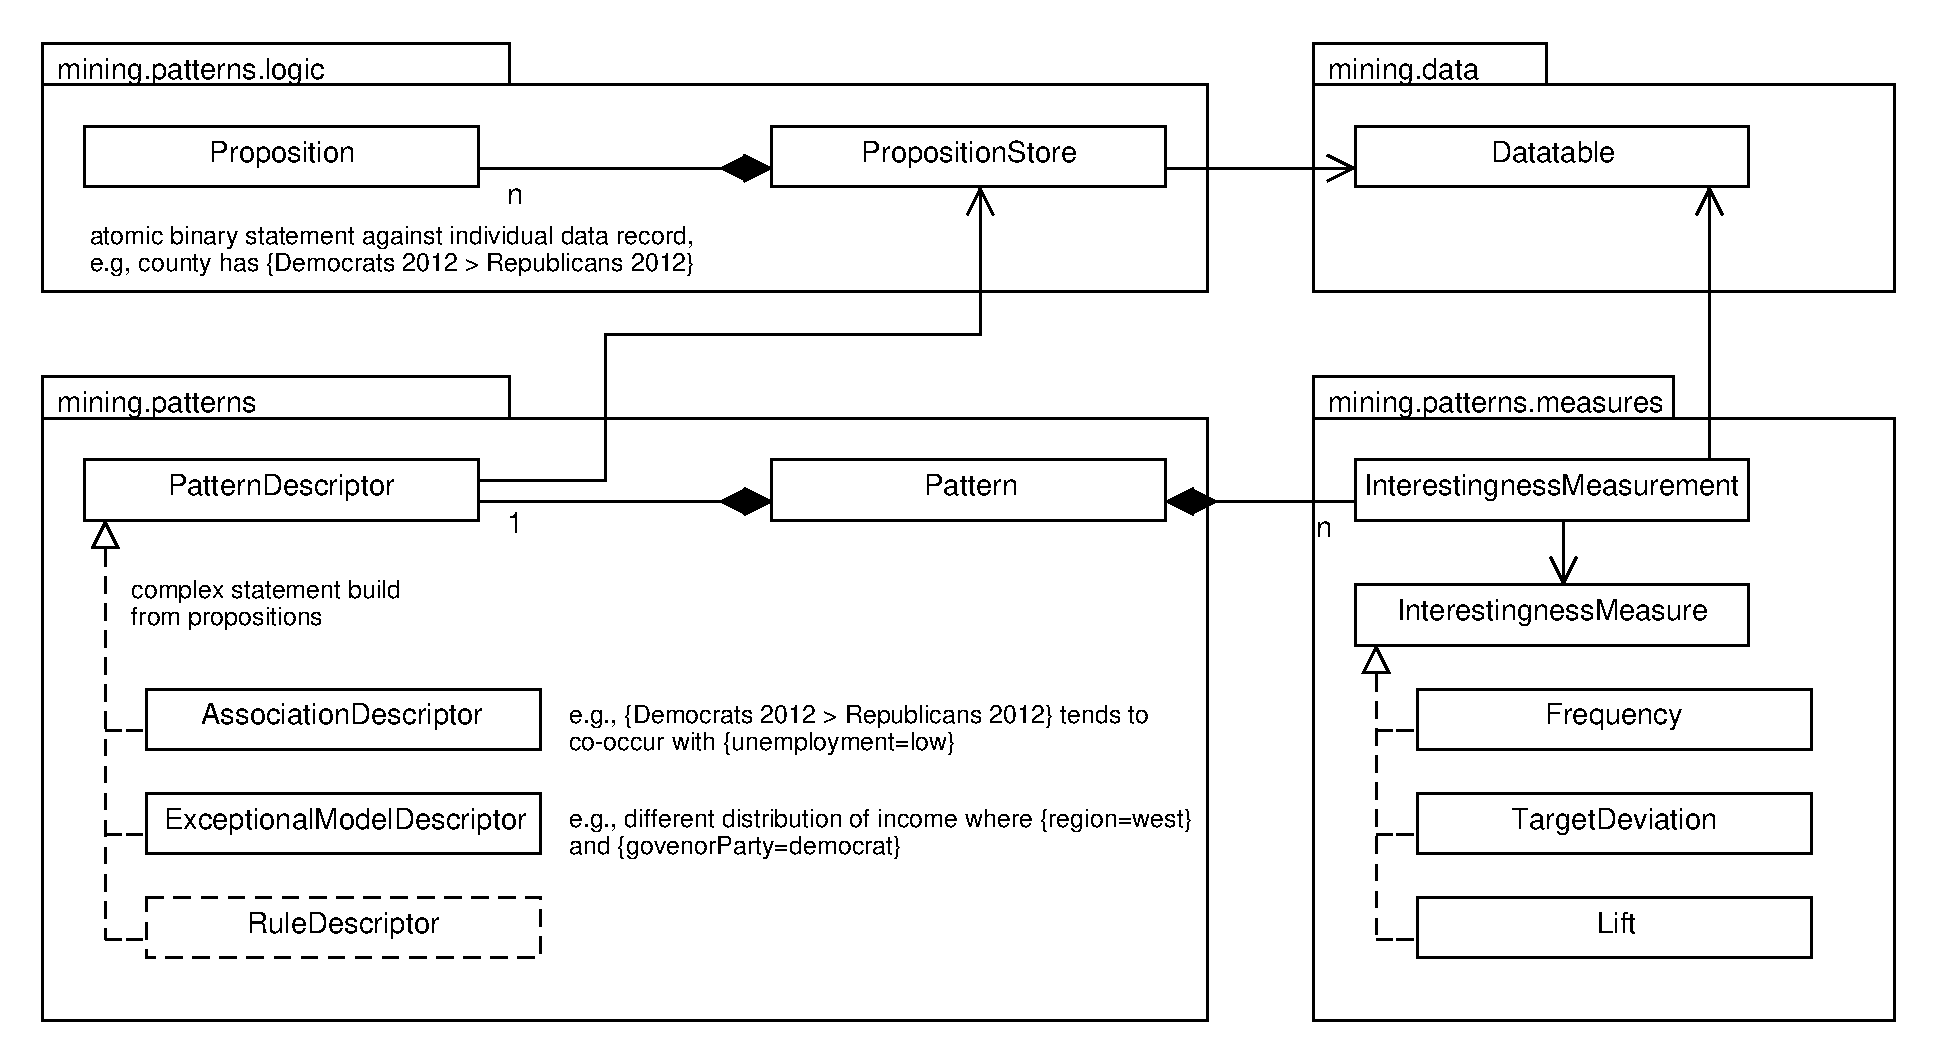
\includegraphics[width=\columnwidth]{mining/patterns.pdf}
\caption{The main classes of the patterns package.}
\end{figure}

Depending on the type of attribute, different statistics can be computed:
category frequencies for categoric attributes, median for ordinal
attributes, and additionally mean, standard deviation, and so on for metric
attributes. This is reflected in the interfaces of the different attribute
sub-types.

\section{Patterns}
Patterns correspond to interesting observations about a dataset that can be
broken down into a) a syntactical statement and b) a rationale supporting the
truth of this statement on a specific dataset of interest. The most abstract
part of the pattern package is the sub-package \class{patterns.propositions}, which defines the classes to express
boolean statements about individual rows of a datatable. Many individual
statements (\class{Proposition}) are aggregated within a
\class{PropositionStore}.
\begin{figure}[ht]
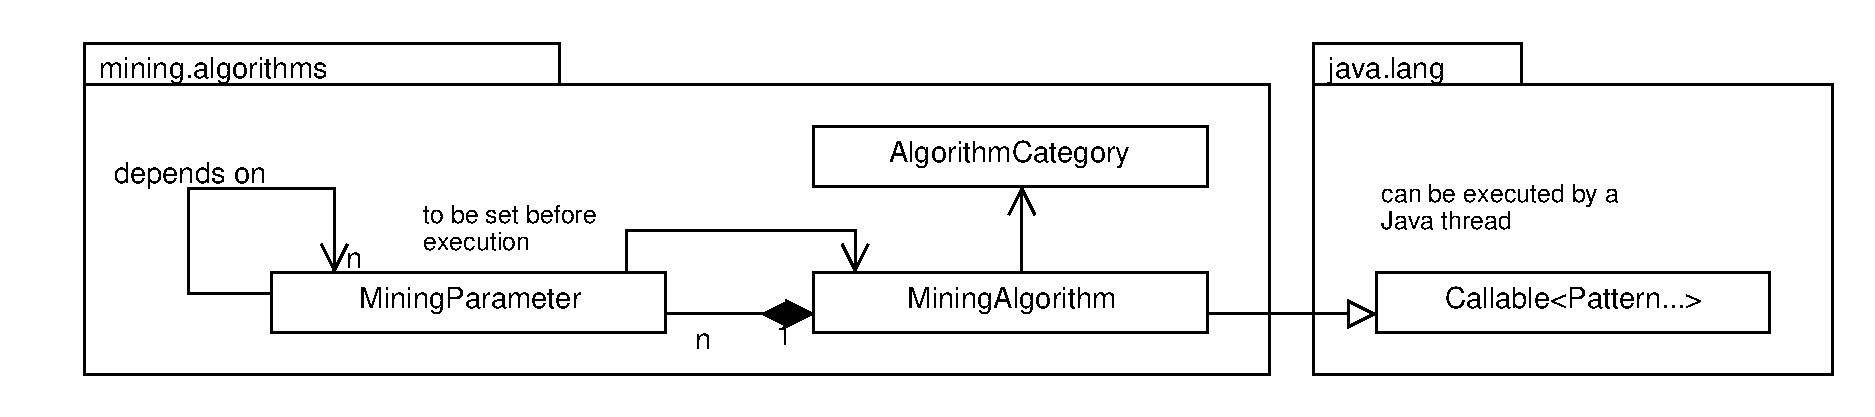
\includegraphics[width=\columnwidth]{mining/algorithms_overview.pdf}
\caption{Main types of the algorithms package.}
\label{fig:alg_overview}
\end{figure}

\section{Algorithms}
Algorithms for pattern discovery are represented by the type
\class{MiningAlgorithm}, which is the main element of the package
\class{mining.algorithms}.
The central functionality of objects of this type is that they can be
\textit{called} in order to produce patterns; and typically this should be
done asynchronously.
Hence, the type is a \class{java.lang.Callable} linking it to standard Java mechanisms.
Additionally, mining algorithms are organized in categories and aggregate
a number of parameters (\class{MiningParameter}), which have to be set to valid values prior to the
execution of the \class{call()}-method (see Fig.~\ref{fig:alg_overview} for an
ontological summary).
Category and parameters provide the means to operate algorithms in a controlled
and documented way to user interfaces and the one-click mining classes.
Note that the contracts of the algorithm and the parameter
java interfaces are coupled.

\subsection{Algorithm Interfaces}
Moving to the interface level (Fig.~\ref{fig:alg_interfaces}) we can see
that the above mentioned functionality of algorithms is actually split across
different interfaces corresponding to the different functionality aspects.
The most basic interface is \class{MiningAlgorithm}, which in addition to the
call-method only provides a boolean method \class{isRunning()}.
This method provides synchronized access to a flag that
indicates if \class{call()} currently is executed in some thread. 
The contract of this level is that \class{call()} is only executed at most in
one thread at a time, which allows this thread to have an exclusive
writing access to almost all of the state of the algorithm object. That is, all
methods that modify the state of the object (except parts that are marked as an
exception in extensions of the interface) have to throw an
\class{IllegalStateException} if they are invoked while
\class{isRunning()==true}---including \class{call()} itself.

\begin{figure}[ht]
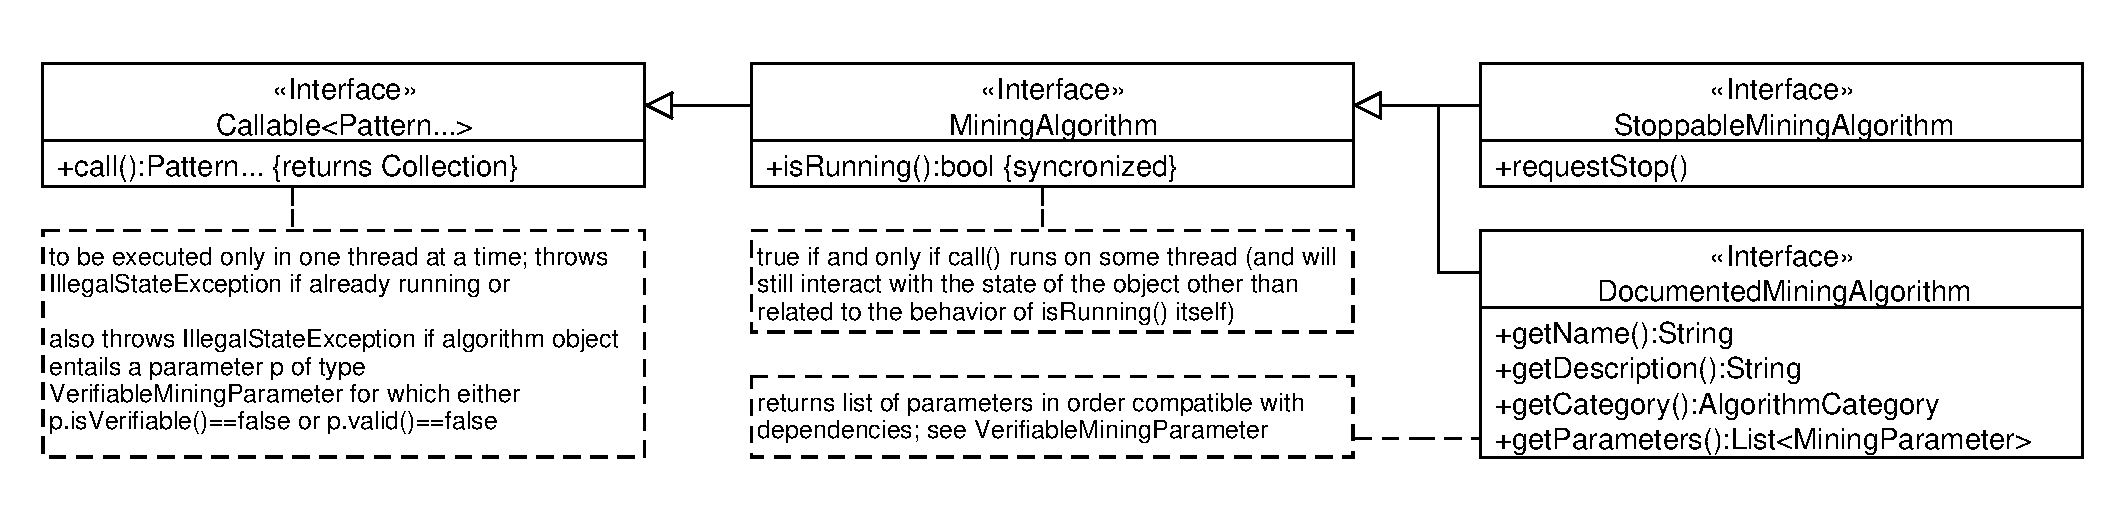
\includegraphics[width=\columnwidth]{mining/algorithms_interfaces.pdf}
\caption{Interfaces of mining algorihms.}
\label{fig:alg_interfaces}
\end{figure}
An optional extension of this interface is \class{StoppableMiningAlgorithm},
which provides the additional void-method \class{requestStop()}. By calling this
method a client can send to an algorithm object the request to stop an execution
of \class{call()} in another thread. Hence, this method is a declared exception
to the above mentioned contract for state-modifying methods in that it does not
throw an exception when the algorithm is running and is allowed to modify a
designated member variable in order to communicate the stop
request to the thread executing \class{call()}. This interface should only be
implemented when also a reasonable handling of stopping requests is provided. In
one-click mining we assume that this is the case for all algorithms.	

The other optional extension of \class{MiningAlgorithm} is
\class{DocumentedMiningAlgorithm}. This interface (along with the interfaces
regarding mining parameters) bundles all the functionality needed to configure
an upcoming run of the \class{call()} method in an informed way and to display
additional meta-information about the algorithm within a graphical user
interface. All non parameter-related meta-information is conveyed by the
methods \class{getName()}, \class{getDescription()}, and \class{getCategory()}, respectively, where the
first two informations are provided as user-readable strings and the latter
takes on values of a small set of algorithmic categories given in the enum
\class{AlgorithmCategory}. These categories are related to the type of patterns
that the algorithm produces, i.e., at the moment they are
\class{ASSOCIATION\_ALGORITHM} and \class{EMM\_ALGORITHM}.
Parameter control and parameter-related meta-information is provided by the
method \class{getMiningParameters}, which returns a list of objects of type
\class{MiningParameter}. This interface is documented in the next subsection.
Note, however, that the contracts of these two parts are coupled. 

\subsection{Parameter Interfaces}
The interface \class{MiningParameter} and its extensions are generics with a
type-parameter \class{T} which represent the type of values that the
parameter can take (see Fig.~\ref{fig:parameters_interfaces}). On the basic
level, the interface allows to retrieve parameter-specific meta-information
(methods \class{getName()}, \class{getDescription()}, and \class{getType()}),
to retrieve the current value (method \class{getCurrentValue()}), and to re-set
the value either by passing a \class{T} (\class{set(T)}) or by a string
representation (\class{setByString(String)}). The last option is provided, e.g.,
for non Java-UIs like Web-UIs, which typically communicate with a browser via
strings. Following the general contract of \class{MiningAlgorithm}, the two
setter-methods have to throw an \class{IllegalStateException} if
\class{isRunning()==true} for the associated algorithm object, which exists for
all \class{MiningParameter} objects. Also note that the current value of a
parameter can be undefined corresponding to \class{getCurrentValue==null}.
\begin{figure}[hb]
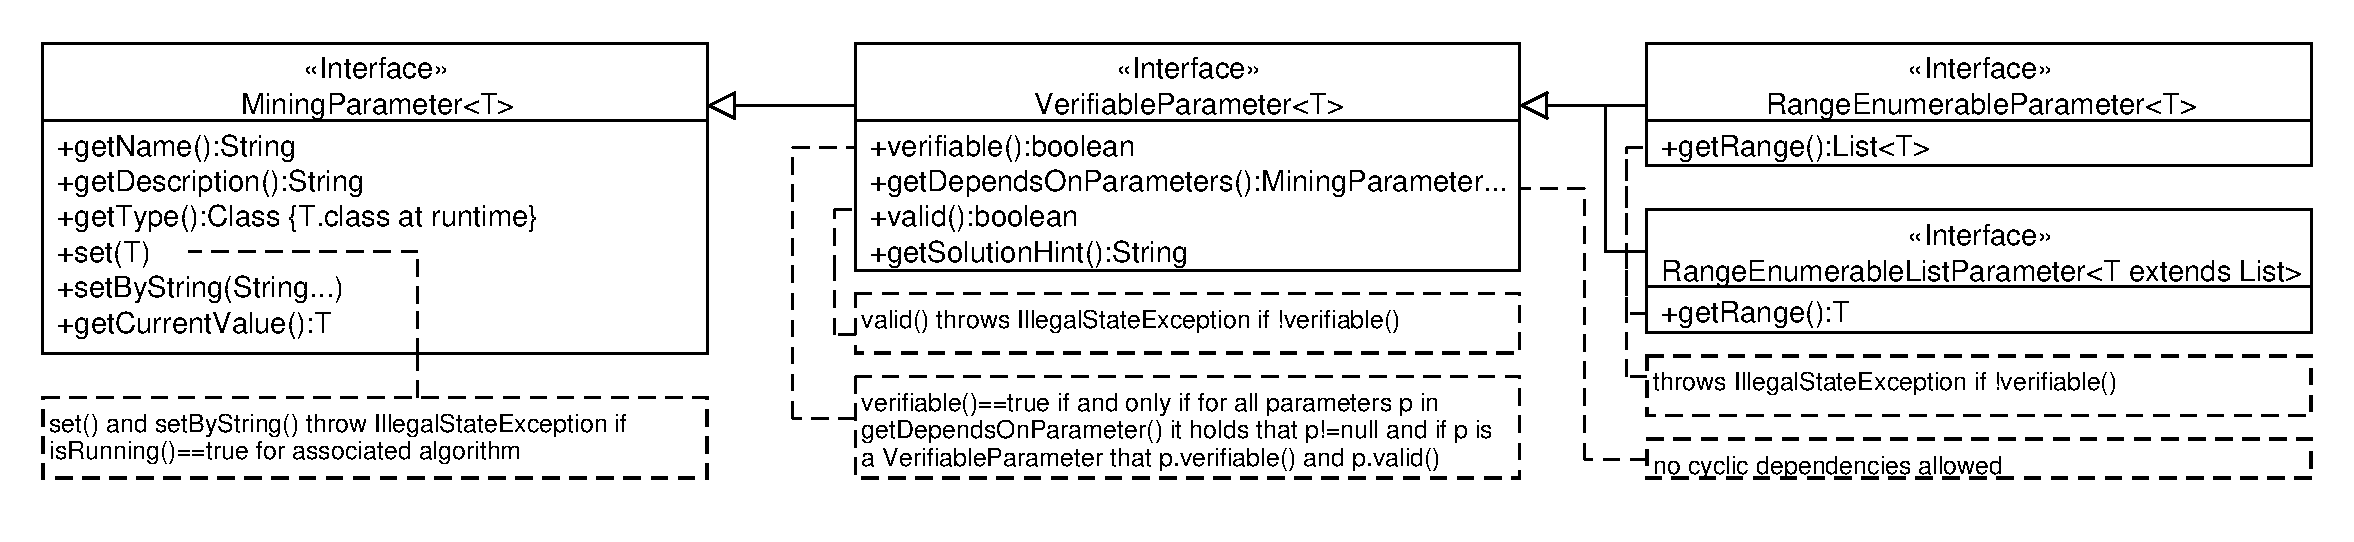
\includegraphics[width=\columnwidth]{mining/parameters_interfaces.pdf}
\caption{Interfaces and implementing classes that represent the mining
algorithms.}
\label{fig:parameters_interfaces}
\end{figure}

While \class{MiningParameter} essentially provides the functionality of a
generic boxed value that respects the contract of \class{MiningAlgorithm}, it
does not provide much support to clients for setting correct values (other
than by providing parameter name and description).
For this purpose, additional functionality is brought in by the interface
\class{VerifiableMiningParameter}. The core method of this interface is the
boolean-valued method \class{valid()} that checks the validity of the currently
set value (as it can be retrieved by \class{getCurrentValue()}). In some use
cases, however, this check can only be performed if already (valid) values have
been set for some other parameters. That is, there can be \emph{dependencies}
between parameters. This dependency structure is available by the method
\class{getDependsOnParameters()}, which returns a list of other mining
parameters.
The validity-check can be performed if for all these parameters \class{p} it holds
that
\begin{itemize}
  \item[a)] \class{p.getCurrentValue()!=null} and
  \item[b)] if \class{p instanceOf Verifiable} then \class{p.valid()==true}.
\end{itemize}
Condition b) implies that the validity-check can be performed for all such
\class{p} recursively referring to their dependencies (hence, no cylcic
dependencies are allowed). As a shortcut, whether the validity-check can be
performed for a parameter can be checked by calling the boolean method
\class{verifiable()}. With these concepts the contract of
\class{MiningAlgorithm} is also extended: \class{call()}
must throw an \class{IllegalStateException} if an algorithm object entails one
\class{VerifiableParameter} which is either not verifiable or not valid.

Finally, there is another two-fold extension of
\class{VerifiableMiningParameter} for cases in which a parameter value cannot only be checked for validity in an
oracle-fashion, but an explicit list of possible values can be given. For this
there are two cases depending on the nature of the type parameter
\class{T} of the mining parameter: 
\begin{itemize}
\item[a)] the parameter can take on a single value from a given list of elements
of type \class{T} or
\item[b)] \class{T} is a
list-type itself, say \class{T=List<U>}; such that the parameter can take on a sub-list of a specified list of elements of type \class{U}.
\end{itemize}
 For case a) the parameter can implement the interface
 \class{RangeEnumerableParameter<T>}, which provides \class{getRange()} with
 return type \class{List<T>}.
 For case b) there is the interface
 \class{RangeEnumerableListParameter<T extends List>}, which provides
 \class{getRange()} with return type \class{T} itself.
 In both cases, the range of valid values can depend on other parameters.
 Hence, \class{getRange()} has the same behavior as \class{valid()} and throws
 an \class{IllegalStateException} in both extensions if the parameter is not verifiable.
 Also, as an additional consistency invariant a
 parameter value is valid if that value is an element from the
 provided list (respectively a sub-list of the provided list in case
 b)). That is, for an instance of \class{RangeEnumerableParameter} with
 \class{verifiable()==true}, it holds that
 \class{valid()==getRange().contains(getCurrentValue())} (with a similar condition for the other case using a sublist check).

% Contributors that implement algorithms for the Pattern
% Discovery API need to respect some standards that are explained in the following.
% 
% \subsubsection{Reacting to request to stop execution}
% Algorithms that are signaled to stop execution should finish as soon as possible.
% The signal needs be queried frequently (e.g. in every internal iteration) and
% should be respected. Continuing execution would not make a difference since results
% generated after the flag is set are not taken into account by result handling.
% 
% \subsubsection{Storing results}
% Algorithms that extend the abstract algorithm base class are provided with a method
% to store the algorithm results. This method should be called whenever new results
% are generated. This applies in particular to results generated \textbf{while} the algorithm
% is running. The method for storing results is thread-safe and lockable.
% Whenever the algorithm is requested to stop, setting new results by the algorithm
% has no effect since the result-container is locked immediately after the stop-signal
% was received.
% 
% \subsubsection{Post-processing}
% Whenever results generated need to be post-processed (e.g. filtering),
% the implementor can override a post-processing method which acts as a hook to achieve that.
% The function is applied to the current set of results when a stop is execution is
% requested. The default implementation just passes the results on, unmodified. If no
% post-processing is needed, the method does not need to be overridden.




\end{document}

